\scanpage{62}
% archive foliation: 61
% lines 1--2
On trouve
\[
\operatorname{Aut}^0(C,a)\simeq\prod_{x\in C_0\setminus\{a\}}
\deleted{\unsure{G_x}}\Pi_x
\]
\figure{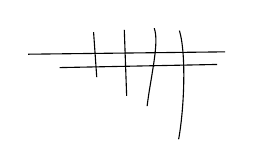
\begin{tikzpicture}[x=1cm,y=1cm]
\draw (0,0)--(2.5,.03);\draw (.4,-.17)--(2.4,-.13);
\draw (.83,.28)--(.87,-.29);\draw (1.22,.31)--(1.25,-.53);
\draw (1.6,.33)..controls(1.67,.15)and(1.55,-.31)..(1.51,-.66);
\draw (1.92,.3)..controls(2.01,0)and(1.98,-.7)..(1.91,-1.08);
\end{tikzpicture}}
% line 3
\deleted{Soit $K$ \unsure{un groupoïde}}
% lines 4--9
Soit $I$ un ensemble muni d'une structure polygonale d'ordre $n\ge2$
\deleted{\unsure{i.e.} $\unsure{\Delta_0}$}
[pour $n=2$, il faut se donner \unsure{l'ens.} des arêtes $I^*$,
\inserted{de cardinal $2$} \deleted{et}
\deleted{cardinal $2$, et}
ou ce qui revient au $=$, $\Omega(\Pi)\simeq I\wedge I^*\ \ldots$],
$\unsure{G|D}$ $(\simeq D_n)$ le \unsure{gpe|groupe} des autom. de $I$.

% lines 10--14
Soit $K=K(I)$ le graphe donné par
\[
\begin{array}{ll}
\uline{\text{Sommets}}:&\unsure{\operatorname{Ob}(\Pi)|\operatorname{Ob}(K)}=C_0=\{o,o'\}\\[4pt]
\uline{\text{arêtes}}&\unsure{I^*|I}\quad(\text{indexation }(\ell_i)_{i\in I})
\end{array}
\]
\deleted{\unsure{Relation d'incidence}}

Incidences : $C_0\times I$ (\unsure{tte} arête incidente à \unsure{tt} \unsure{sommet|sommets})
% lines 15--17, interlinear addition
\inserted{$G$ opère sur $K(I)$, et on a aussi l'\uuline{involution} $\tau$
qui est l'identité sur $I$, et échange $o,o'$, commutant à $G$.}
% lines 18--22 and left drawing
\begin{minipage}{.24\linewidth}
\figure{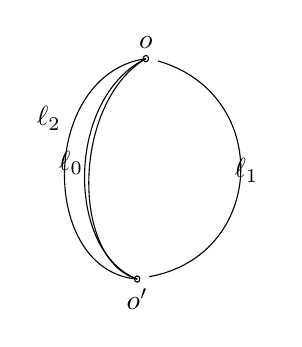
\begin{tikzpicture}[x=.85cm,y=1cm]
\coordinate (a) at (1,2.8);\coordinate (b) at (.87,0);
\draw (a)..controls(-.6,2.6)and(-.6,.1)..(b);
\draw (a)..controls(-.2,2.3)and(-.2,.35)..(b);
\draw (a)..controls(-.1,2.25)and(-.13,.25)..(b);
\draw (1.18,2.77)..controls(2.9,2.35)and(2.8,.3)..(1.05,.03);
\draw (a) circle(.04);\draw(b)circle(.04);
\node[above]at(a){$o$};\node[below]at(b){$o'$};
\node at(-.45,2.04){$\ell_2$};\node at(-.12,1.48){$\ell_0$};\node at(2.5,1.38){$\ell_1$};
\end{tikzpicture}}
\end{minipage}\hfill
\begin{minipage}{.72\linewidth}
Soit $C(I)$ le groupoïde fondamental de $K(I)$.
\deleted{le groupe} $G$ y opère par automorphismes, en opérant transitivement sur $C_0=\{o\ o'\}$.
\end{minipage}

% line 23
On va regarder le \deleted{commutant}\inserted{normalisateur de $G$} dans
